\chapter{BACKGROUND}
\label{chap:bg}

\section{Goal Models}
\label{sec:bg:gm}
Goal Models are used in representing one or more goals. These goals are obtained from a system or its stakeholders. Goals often have relationships to other goals describing its impact or how they can be achieved. The primary aim of a goal model is to enhance the likelihood of a system's success by warranting that the software has a significant role in a complex socio-technical system. To augment this goal models allow explicit consideration of the system or its stake holders in the Requirements Engineering Process, there by allowing business analysts to assure that all the required goals are satisfied and all the proposed design alternatives or feature decisions satisfy the domain requirements. Goal Modeling is applied in multiple industrial systems like air traffic management \cite{maiden04}, non-profit organizations \cite{horkoff09} and health care domains \cite{anY09}. There are multiple goal modeling frameworks, techniques and methodologies. The remaining paragraphs in this section highlight few popular goal modeling frameworks.

\subsection{KAOS}
\label{subsec:bg:gm:kaos}
KAOS(\textit{\textbf{K}nowledge \textbf{A}cquisition in aut\textbf{O}mated \textbf{S}pecification}) is one of the first proposed Goal Modeling approaches \cite{van09} and is popular in eliciting, modelling and reasoning system requirements. The KAOS model contains two primary components, \textit{Goals} \& \textit{Agents}. Goals are prescriptive statements of intent that the system should satisfy through the cooperation of its agents, while agents are active system components playing specific roles in the satisfaction of goals. Goals are further refined into sub-goals through \textit{AND/OR} dependencies.
\begin{itemize}
    \item \textbf{AND}: Satisfaction of all of the sub-goals ensures satisfaction of the parent goal.
    \item \textbf{OR}: Satisfaction of either of the sub-goals ensures satisfaction of the parent  goal.
\end{itemize}

\begin{figure}[hbtp]
    \centering
    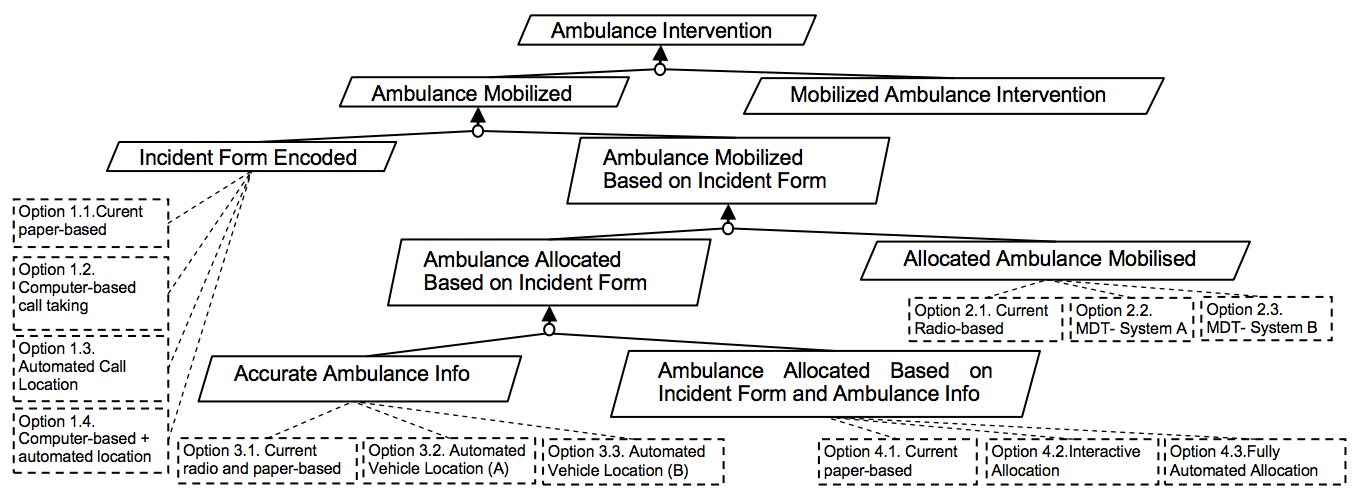
\includegraphics[width=\textwidth]{Chapter-2/figs/KAOS}
    \caption{Partial Goal Model for LAS.}
    \medskip
    \small
    Originally from \cite{heaven11}.
    \label{fig:kaos}
\end{figure}

An example of the KAOS model is shown in \fref{fig:kaos}, depicting a portion of a goal model built for the London Ambulance Service(LAS) case study \cite{finkelstein96}. The top level goal in the figure \textit{``Ambulance Intervention"} has 2 AND dependencies and requires both of them to be satisfied. One of the bottom level goals ``Accurate Ambulance Info" contains 3 OR dependencies and needs only one of them to be satisfied.

Although the KAOS model provides completeness to the requirements documents and traceability between the problem description and solution description, it suffers from few important deficiencies.
\begin{itemize}
    \item KAOS does not model the strategic relationship between the stakeholders.
    \item In situations where the Goals are not quantitative, the relationship between Goals and Agents cannot be categorized using AND and OR dependencies.
\end{itemize}

\subsection{GBRAM}
\label{subsec:bg:gm:gbram}

\begin{figure}[hbtp]
    \centering
    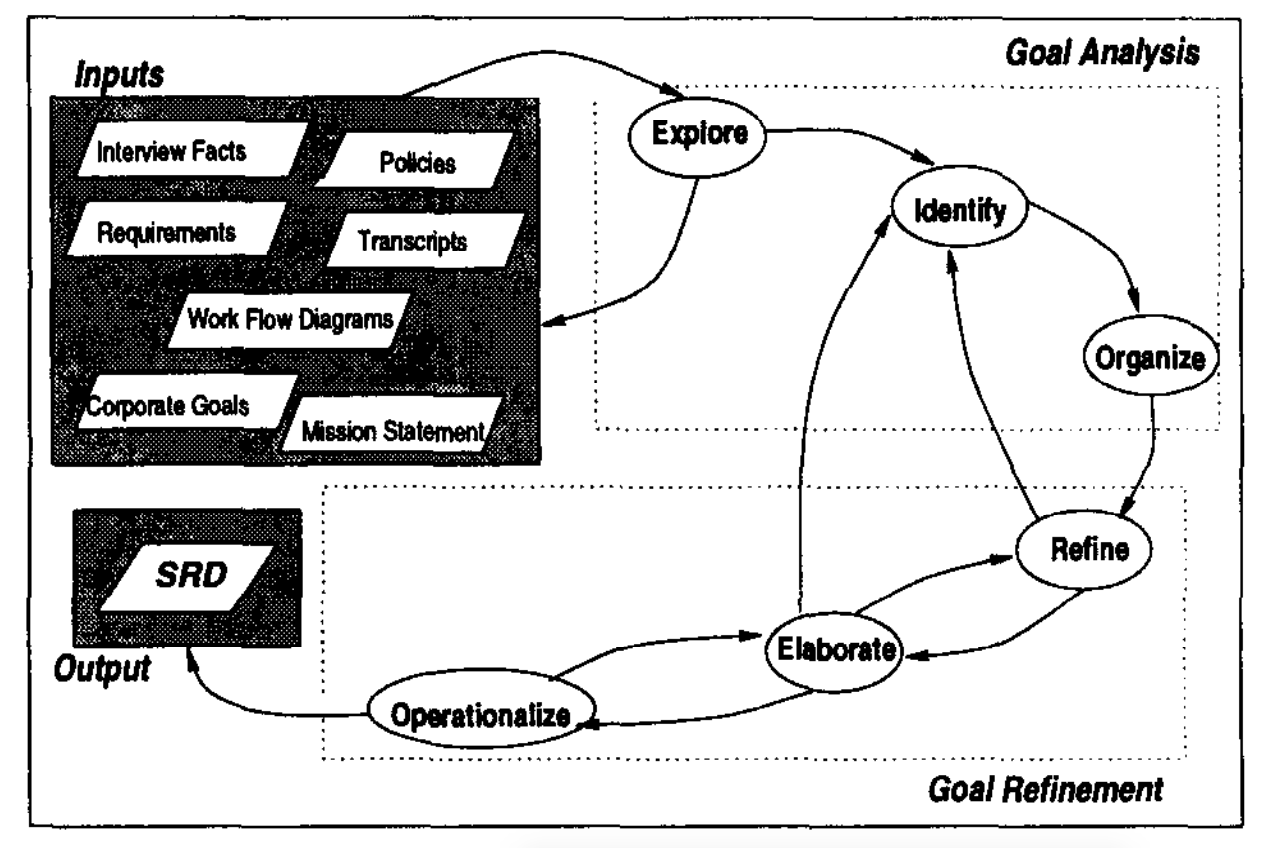
\includegraphics[width=\textwidth]{Chapter-2/figs/GBRAM}
    \caption{Activities in GBRAM.}
    \medskip
    \small
    Originally from \cite{anton98}.
    \label{fig:gbram}
\end{figure}

Anton Et al. proposed GBRAM(\textit{\textbf{G}oal \textbf{B}ased \textbf{R}equirements \textbf{A}nalysis \textbf{M}ethod}) \cite{anton98} which is based on the assumption that goals have not been documented previously and that analysts need to work from different sources of information. \fref{fig:gbram} summarized the two components of GBRAM.\\
\textbf{Goal Analysis:}
\begin{itemize}
    \item \textit{Explore} activities based on available information.
    \item \textit{Identify} activities by extracting goals and the corresponding agents.
    \item \textit{Organize} activities by classifying goals and organizing them based on their dependencies.
\end{itemize}

\textbf{Goal Refinement:}
\begin{enumerate}
    \item \textit{Refine} activities by pruning the set of goals.
    \item \textit{Elaborate} the process of analyzing the goal set by considering possible goal obstacles and constructing scenarios to uncover hidden goals and requirements.
    \item \textit{Operationalize} goals by translating requirements for the final requirements specification.
\end{enumerate}

Like the KAOS model in section \ref{subsec:bg:gm:gbram}, GBRAM suffers from the same problems although the framework introduces the concept of constraints the highlight the relationship between the goals.

\subsection{NFR}
\label{subsec:bg:gm:nfr}

The NFR(\textit{\textbf{N}on-\textbf{F}unctional \textbf{R}equirement}) modeling framework is designed to represent user intentions in technical systems \cite{chung00}. 
An NFR is a type of requirement which is used to evaluate the operation of the system rather than its behaviour based on specific criteria.

The NFR framework decouples the concept  of functionality from other attributes used to justify quality and concerns for productivity, time and cost using a higher level abstraction. Rather than focusing on expressing requirements in the form of descriptive functions, constraints and attributes, NFR uses the concept of \textit{softgoals} which are not satisfied through clear-cut criteria. The framework also incorporates AND and OR decompositions amongst goals and contribution links which represent (partially)positive and (partially) negative contributions to and from softgoals.

The NFR framework addresses the one of the drawbacks of KAOS and GBRAM by using softgoals where dependencies can now be represented as contributions. But the problem of the ``strategic relationship amongst stakeholders" still persists.

\subsection{i*}
\label{subsec:bg:gm:istar}
The i* framework \cite{yu97} is utilizes the key concepts of NFR framework, including softgoals, AND/OR decompositions and contribution links along with goals, resources and tasks. The model addresses the prime drawback of its predecessors by including dependencies between actors(agents).

The i* framework describes dependencies among actors. There are four primary elements to describe the model: \textbf{goal}, \textbf{soft goal}, \textbf{task} and \textbf{resource}. Intentional actor forms the central concept in i*. Organizational actors are viewed as having intentional properties such as goals, beliefs, abilities, and commitments (concept of distributed intentionality). Actors depend on each other for goals to be achieved, tasks to be performed and resources to be generated. By depending on others, an actor may be able to achieve goals that are difficult or impossible to achieve on its own. On the other hand, an actor becomes vulnerable if the actors it depended on did not deliver. Actors are strategic in the sense that they are concerned about opportunities and vulnerabilities, and seek rearrangement of their environments that would better serve their interests by restructuring intentional relationships.

\fref{fig:istar} depicts a sample i* Model for youth counselling. Hexagons represent Tasks; Goals are represented by ellipses; Rectangles represent resources; and Softgoals are represented by the informal shapes.

\begin{figure}[hbtp]
    \centering
    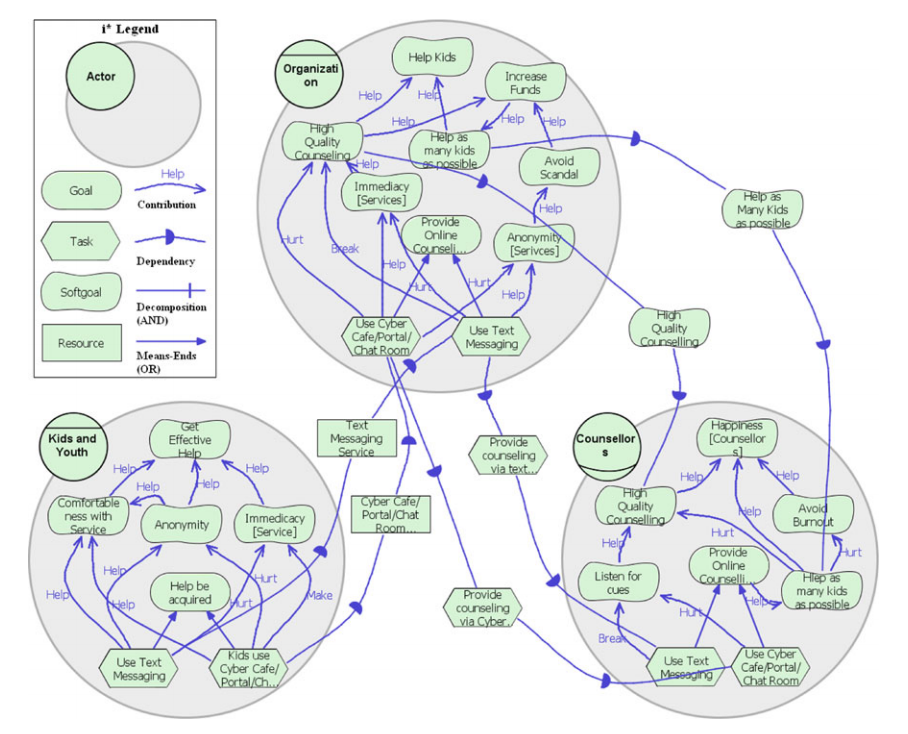
\includegraphics[width=\textwidth]{Chapter-2/figs/istar}
    \caption{Sample i* Model for youth counseling}
    \medskip
    \small
    The legend on the top left indicates the legend for all the components of the i*. Originally from \cite{horkoff12}.
    \label{fig:istar}
\end{figure}


The i* model is very verbose and one of the prime models used in Requirements Engineering. A reduced form the i* model is used in GRL(goal oriented language)\cite{amyot10} and it is also the first stage of TROPOS \cite{giorgini05}, an agent oriented system development methodology.

\subsection{AHP}
\label{subsec:bg:gm:ahp}

The AHP(\textit{\textbf{A}nalytic \textbf{H}ierarchy \textbf{P}rocess}) modelling framework was developed by Thomas Saaty in 1987 for organizing and analyzing complex decisions based on mathematics and psychology \cite{saaty87}. AHP is used extensively in applications like group decision making in fields such as government, business, industry, healthcare, ship building and education \cite{saracoglu13}.

\begin{table}[htbp]
\centering
\begin{tabular}{|c|l|l|}
\hline
\textbf{Scale} & \multicolumn{1}{c|}{\textbf{\begin{tabular}[c]{@{}c@{}}Definition (in terms \\ of Importance)\end{tabular}}} & \multicolumn{1}{c|}{\textbf{Comment}} \\ \hline
1 & Equal & Two activities contribute equally to the objective \\ \hline
2 & Weak & \multirow{2}{*}{\begin{tabular}[c]{@{}l@{}}Experience and judgement slightly favor one \\ activity over another.\end{tabular}} \\ \cline{1-2}
3 & Moderate &  \\ \hline
4 & Moderate plus & \multirow{2}{*}{\begin{tabular}[c]{@{}l@{}}Experience and judgement strongly favor one \\ activity over another.\end{tabular}} \\ \cline{1-2}
5 & Strong &  \\ \hline
6 & Strong plus & \multirow{2}{*}{\begin{tabular}[c]{@{}l@{}}An activity is favored very strongly demonstrated\\ over another.\end{tabular}} \\ \cline{1-2}
7 & Very strong &  \\ \hline
8 & Very very strong & \multirow{2}{*}{\begin{tabular}[c]{@{}l@{}}The evidence favoring one activity over another\\ is of the highest possible order of assumption.\end{tabular}} \\ \cline{1-2}
9 & Extreme &  \\ \hline
\begin{tabular}[c]{@{}c@{}}Reciprocals\\ of above\end{tabular} & Inverse Relation & \begin{tabular}[c]{@{}l@{}}If activity i has one of theabove non-zero numbers\\ assigned to it when compared with activity j, then\\ j has the reciprocal value when compared with i.\end{tabular} \\ \hline
1.1 - 1.9 & Activities are very close & \begin{tabular}[c]{@{}l@{}}Contrasting activities with the size of small numbers\\ with relative importance of activities.\end{tabular} \\ \hline
\end{tabular}
\caption{Scale of priorities used for comparison}
\label{tab:ahp:props}
\end{table}

Saaty described the process of making decisions using AHPs as follows:

\begin{enumerate}
    \item The problem is defined and the kind of knowledge to be sought is determined.
    \item The hierarchy of decisions from the top with the goal of the decision is structured, following which the objectives are structured from a broad perspective though the intermediate levels(factors on which subsequent elements depend) to the lowest level(set of alternatives).
    \item A set of pairwise comparison matrices are constructed. Each element in a higher level is used to compare the elements in the level immediately below with respect to it.
    \item The priorities obtained from the comparisons are used to weight the priorities in the level immediately below. This is repeated for every element. For each element in the level below its weighed values are added and its overall or global priority is obtained. This process of weighing and adding is continued until the final priorities of the alternatives in the bottom most level are obtained.
\end{enumerate}


For the purpose of making comparisons, a scale of numbers that indicates how many times more important or dominant one element is over another element with respect to the criterion or property against which the elements are compared. This scale is highlighted and explained in \tref{tab:ahp:props}.


\section{Multi-Objective Optimization}
\label{sec:bg:moo}

A \textbf{M}ulti-\textbf{O}bjecitve \textbf{O}ptimization(MOO) is a category of mathematical optimization problem which involves more than one objective function to be optimized simultaneously. Mathematically, a MOO can be defined as follows
\begin{equation}
    \begin{aligned}
        & minimize \quad F(x) = (f_1(x), \ldots ,f_m(x))  \\
        & subject\ to \quad x \in \Omega
    \end{aligned}
    \label{eq:MOO}
\end{equation}


where $\Omega$ is the \textit{decision (variable) space}, $R^m$ is the objective space and $F : \Omega \rightarrow R^m$ consists of $m$ real-valued objective functions. If $\Omega$ is a closed and connected region in $R^n$ and all the objectives are continuous of $x$, the problem in \eref{eq:MOO} is categorized as a \textit{Continuous Multi-Objective Optimization Problem}.

Let $a = (a_1, \ldots , a_m), b = (b_1, \ldots , b_m) \in R^m$ be two vectors, then $a$ is said to \textit{dominate} $b$ if $a_i \leq b_i$ for all $i = 1, \ldots, m$, and $a \neq b$.\footnote{This is described for a minimization problem. All the inequalities is reversed to maximize the objective in \cite{miettinen99}. ``Dominate" refers to ``better than".} A point $x^* \in \Omega$ is called \textit{(globally) Pareto optimal} if there is no $x \in \Omega$ such that $F(x)$ dominates $F(x*)$. The set of all the Pareto optimal points is called the \textit{Pareto Set}($PS$). The set of all the Pareto objective vectors is defined as $PF = \{ F(x) \in R^m | x \in PS\}$, is called the \textit{Pareto Front}\cite{miettinen99}.

None of the points on the Pareto front can be said to better than another. This raises a need to find as many Pareto Optimal points as possible. Classically, optimization methods like Simulated Annealing \cite{kirkpatrick83}, Particle Swarm Optimization \cite{kennedy95} and other evolutionary methods\cite{fonseca93} converted the multi-objective optimization problem to a single-objective optimization problem by emphasizing one particular Pareto-optimal solution at a time. Using such methods to find the Pareto Front, the method needs to be applied multiple times with the hope of finding a different point for each simulation run.


\section{Literature Review}
\label{sec:bg:lr}

\subsection{Interactive Analysis}
\label{subsec:bg:lr:interactive}
An interactive goal model analysis was performed by Horkoff Et. al\cite{horkoff12} based on \textit{Forward} and \textit{Backward} Propagation techniques. In forward propagation, the ``satisfaction level" of the goals is propagated onto other goals on the paths of the contributions as defined on the model. On the other hand in the backward propagation method, the model is traced back onto the potential solutions and subsequent goals are checked for their satisfiability by asking questions of the models. While questions are analyzed alternative paths are also considered to satisfy a node. Although this method is highly effective, there is a large amount of human involvement particularly in case of conflicts or cycles in the model which results in constant interruptions. Moreover, the approach also fails to enlist different possible optimum solutions in a single execution run. For a different expected output, the stakeholder has to provide a different input when prompted, thus making the approach cumbersome in case of complex models.

\subsection{Partial Goal Satisfaction Reasoning}
\label{subsec:bg:lr:parGoalSat}
Letier Et. al \cite{letier04} developed an extension of the KAOS  \cite{van09} for reasoning about alternative design choices based on measurable, domain-specific criteria.  In this framework, the degrees of satisfaction for a goal are specified using objective functions defined in terms of quality variables, which are random variables (i.e. functions over probability spaces). For example, they specify the goal Achieve [Ambulance Intervention] from \fref{fig:kaos} in \fref{fig:pgsr}.

\begin{figure}[!hbtp]
    \begin{mdframed}
        \noindent
        \textbf{Goal} Achieve[Ambulance Intervention] 
        
        \noindent
        \textbf{Definition}
        
        \noindent
        For every urgent call reporting an incident, there should be an ambulance at the incident scene within 14 minutes after receiving the first call.
        
        \noindent
        \textbf{Formal Definition}($\forall i:Incident, c:UrgentCall$)
        
        $Reporting(c,i) \implies \diamond_{14mins} (\exists a:Ambulance) Intervention(a,i)$
        
        \noindent
        \textbf{Objective Functions}
        
        $14MinResponseRate = MAX[P(ResponseTime \leq 14 mins)]$
        
        $8MinResponseRate = MAX[P(ResponseTime \leq 8 mins)]$
        
        \noindent
        \textbf{Quality Variable}
        
        $ResponseTime: Incident \rightarrow Time$
        
        \{\textbf{def:} the duration in seconds between the start of the first call reporting the incident and the 
        
        arrival of the first ambulance at the incident scene.\}    
    \end{mdframed}
    
    
    \caption{Quantitative Goal Model Representation for London Ambulance Service}
    \label{fig:pgsr}
\end{figure}



The goal's definition and formal definition define what it means for the goal to be satisfied in an absolute sense; the goal semantic is the set of system behaviours – i.e. sequences of system states – that satisfy the goal's formal definition. The goal objective functions define the measures to be used for assessing partial levels of goal satisfaction. Objective functions are defined in terms of quality variables that correspond to domain phenomena related to the goal's definition. The quality variables associated with a goal can be related to quality variables associated with its sub-goals through domain-specific \textit{refinement equations}. 

This approach exibits the same problem as that of the Interactive model i.e the approach also fails to enlist different possible optimum solutions in a single execution run.


\subsection{Simulation \& Optimization}
\label{subsec:bg:lr:simOpt}

Heaven Et. al \cite{heaven11} overcame these drawbacks by presenting a simulation and optimization framework for evaluating the impact of alternative system decisions on high level goals and for finding optimal decision. The simulation model is then used by a multi-objective optimization component that searches through the design space in order to identify the optimal decision choices. NSGAII\cite{deb02} was their choice of multi-objective optimization algorithm used to search the decision space. Although the approach catered to obtaining a wide range of optimal solutions, it failed when the number of competing requirements exceeded three objectives or for highly constrained models.


% \section{Tables}
% Table \ref{tab:one} is about as simple as they come, to put a formula in a 
% table just use the same methods as putting a formula in a paragraph.  
% Table \ref{tab:two} is a similar table in landscape on a seperate page.  
% %
% \begin{table}
% \caption{Table Example}
% \label{tab:one}
% \begin{center}
% \begin{tabular}{lccl}
% \toprule
% Treatment & No Death & Death & Total\\
% \midrule
% Therapy A & 1295 & 72 & 1367\\
% Therapy B 	& 2294 & 195 & 2489\\
% \midrule
% Total & 3589 & 267 & 3856\\
% \bottomrule
% \end{tabular}
% \end{center}
% \end{table}

% \paragraph{Filler Text} \lipsum[1-2]
% \newgeometry{margin=1in,lmargin=1.25in,footskip=\chapterfootskip, includehead, includefoot}
% %\thispagestyle{lscape}
% %\pagestyle{lscape}
% \thispagestyle{lscapedplain}
% \begin{landscape}
% \begin{table}
% \caption{Landscape Table Example}
% \label{tab:two}
% \begin{center}
% \begin{tabular}{lcccccccccl}
% \toprule
% Patient & A & B & C & D & E & F & G & H &I & Total \\
% \midrule
% John & 1 & 2 & 3 & 4 & 5 & 6 & 7 & 8 & 9 & 45 \\
% Amy & 1 & 2 & 3 & 4 & 5 & 6 & 7 & 8 & 9 & 45 \\
% Jim & 1 & 2 & 3 & 4 & 5 & 6 & 7 & 8 & 9 & 45 \\
% Jason & 1 & 2 & 3 & 4 & 5 & 6 & 7 & 8 & 9 & 45 \\
% Sandy & 1 & 2 & 3 & 4 & 5 & 6 & 7 & 8 & 9 & 45 \\
% Icem & 1 & 2 & 3 & 4 & 5 & 6 & 7 & 8 & 9 & 45 \\
% \midrule
% Total & 6 & 12 & 18 & 24 & 30 & 36 & 42 & 48 & 54 & 270\\
% \bottomrule
% \end{tabular}
% \end{center}
% \end{table}
% \end{landscape}
% %\newgeometry{margin=1in,lmargin=1.25in,footskip=\chapterfootskip, includehead, includefoot,landscape=false}
% \restoregeometry
% \pagestyle{fancy}
% \thispagestyle{fancy}
% \newgeometry{margin=1in,lmargin=1.25in,footskip=\chapterfootskip, includehead, includefoot}


% \section{Figures}

% The easiest way to insert a picture is to have that picture in pdf format.  
% \fref{fig:hist1} and \fref{fig:hist2} are two figures typeset normally.
% ETD guidelines allow the use of landscape pages in the electronic 
% submission.  To rotate a page, do NOT use the \texttt{lscape} environment. Instead, use the \texttt{pdflscape} package, for compatibility with PDFlatex.
% Please note, if you are preparing a document for binding, consider
% giving the \texttt{hardcopy} option in the \verb|\documentclass|
% declaration.  This will place the page number at the normal location,
% which is where it should be for printing and binding.
% %
% \begin{figure}[hbtp]
% \centering
% 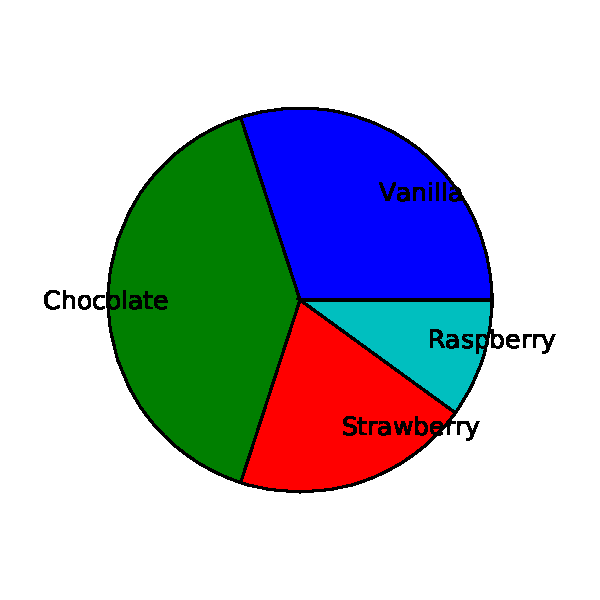
\includegraphics[width=0.6\textwidth]{Chapter-2/figs/pie}
% \caption{Here is a sample figure}
% \label{fig:hist1}
% \end{figure}

% For an example of a figure with a really long caption, see Fig.~\ref{fig:longcap}
% \begin{figure}[hbtp]
% \centering
% \calculategraphicstargetheight{11}
% 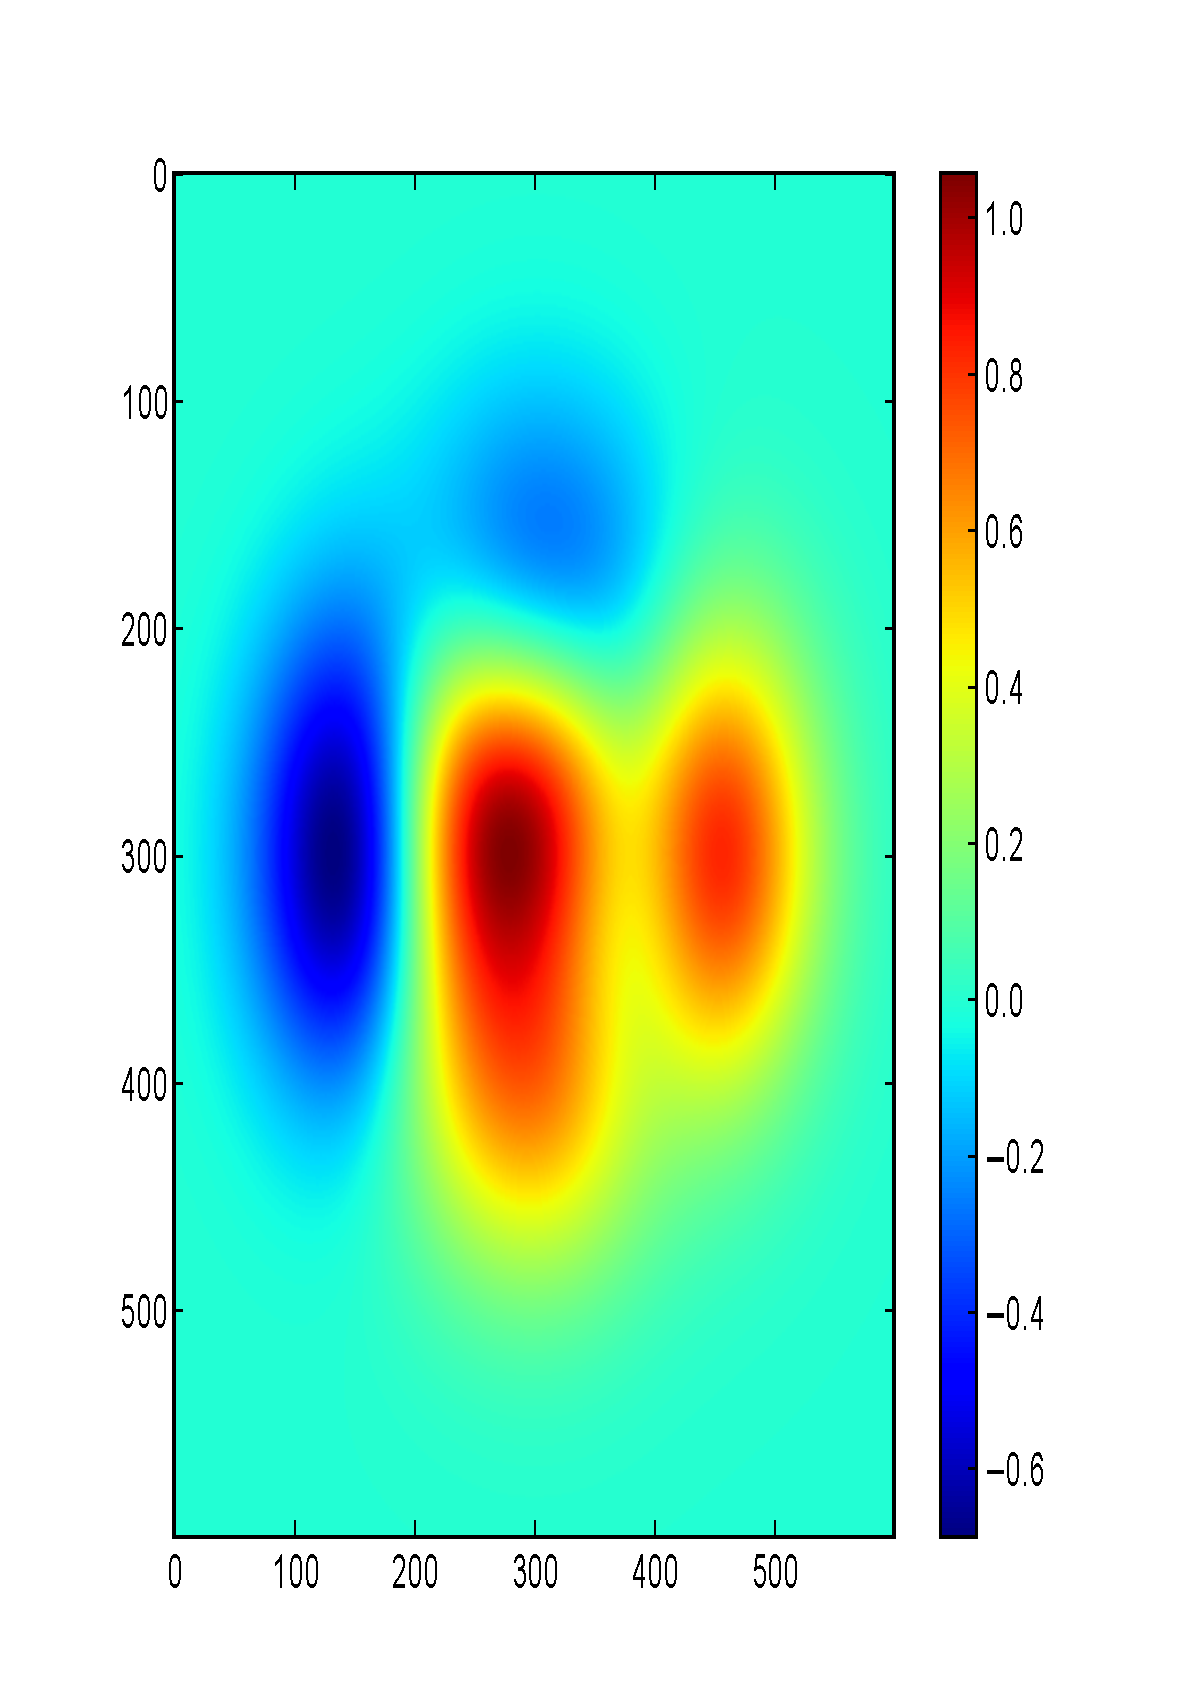
\includegraphics[height=\graphht]{Chapter-2/figs/color_stretched}
% \caption{Here is a HUGE sample figure with a HUGE caption. Our goal is to make a caption that is so long that the caption spills into the lower margin, leading to an ETD error. The way to solve this problem in a systematic way is to calculate how many lines of text the caption will use, then adjust the size of the image, such that it leaves just enough space for your huge caption. How I am solving this problem is by providing a new variable called graphht that stores how tall the image should be. Then, to calculate how tall to make the figure, you use the new function that I am providing called calculategraphicstargetheight. This function has one argument. The argument of the function is how many lines of text you estimate that the caption occupies. You can always run your tex once, measure this number, and type it into the argument for the function. What the function will do (it is defined in the preamble) is take into account the size you give it, the spacing of the chapter and the footer at the bottom, 
% and then calculate the total vertical space available. Thus, this function should be used for images that are taller than they are wide.}
% \label{fig:longcap}
% \end{figure}
% %
% \begin{figure}[hbtp]
% \centering
% 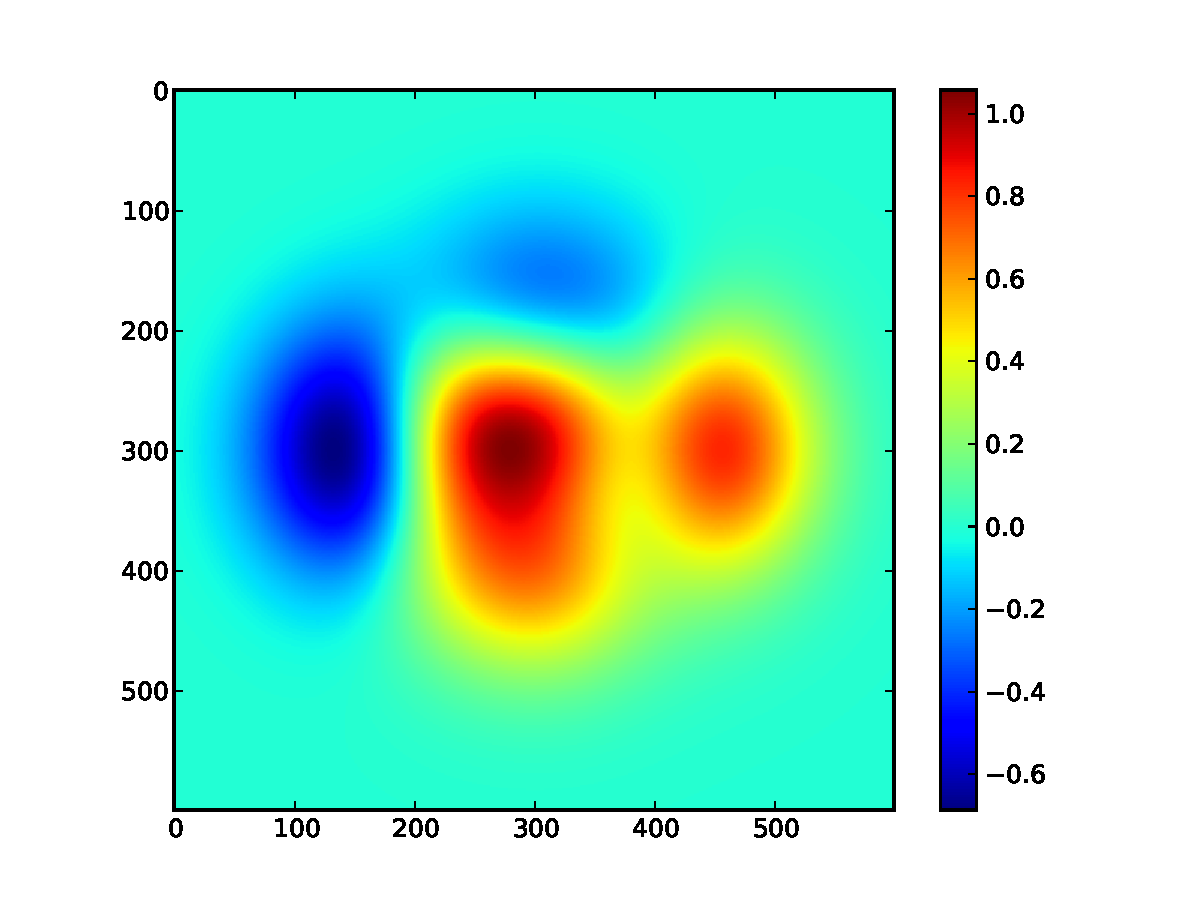
\includegraphics[width=0.6\textwidth]{Chapter-2/figs/color}
% \caption{Here is a sample figure}
% \label{fig:hist2}
% \end{figure}
% %
% \begin{figure}[hbtp]
% \centering
% \subfloat[]{
% 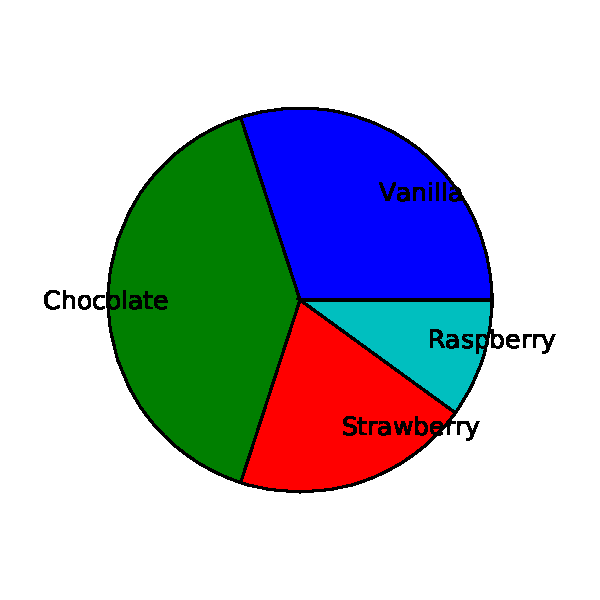
\includegraphics[width=0.4\textwidth]{Chapter-2/figs/pie}
% }
% \subfloat[]{
% 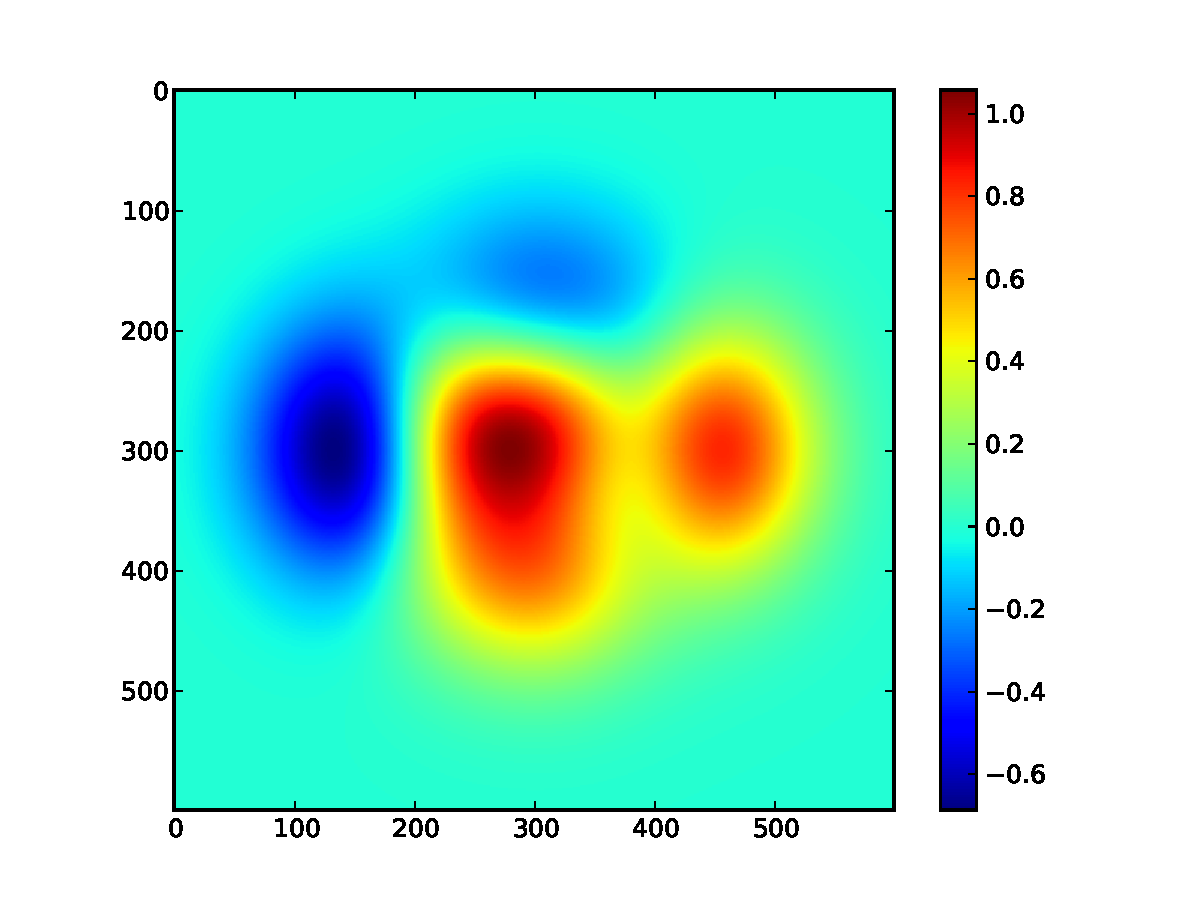
\includegraphics[width=0.4\textwidth]{Chapter-2/figs/color}
% }
% \caption{Here are two floating subfigures}
% \label{fig:subfigures}
% \end{figure}


% \paragraph{Filler Text} \lipsum[12-15]

% \newgeometry{margin=1in,lmargin=1.25in,footskip=\chapterfootskip, includehead, includefoot}
% %\thispagestyle{lscaped}
% %\pagestyle{lscaped}
% \thispagestyle{lscapedplain}
% \begin{landscape}
% \begin{figure}
% \centering
% 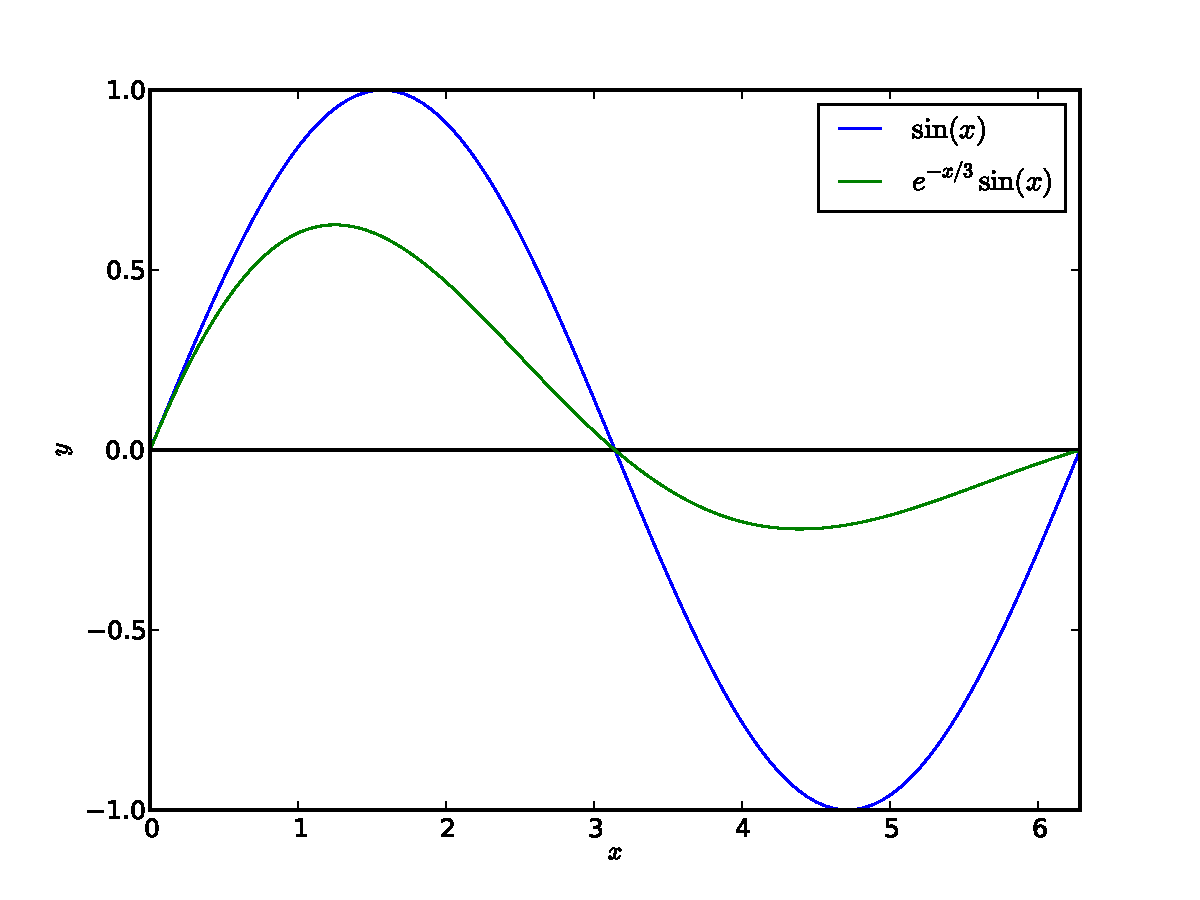
\includegraphics[width=\textwidth]{Chapter-2/figs/sine}
% %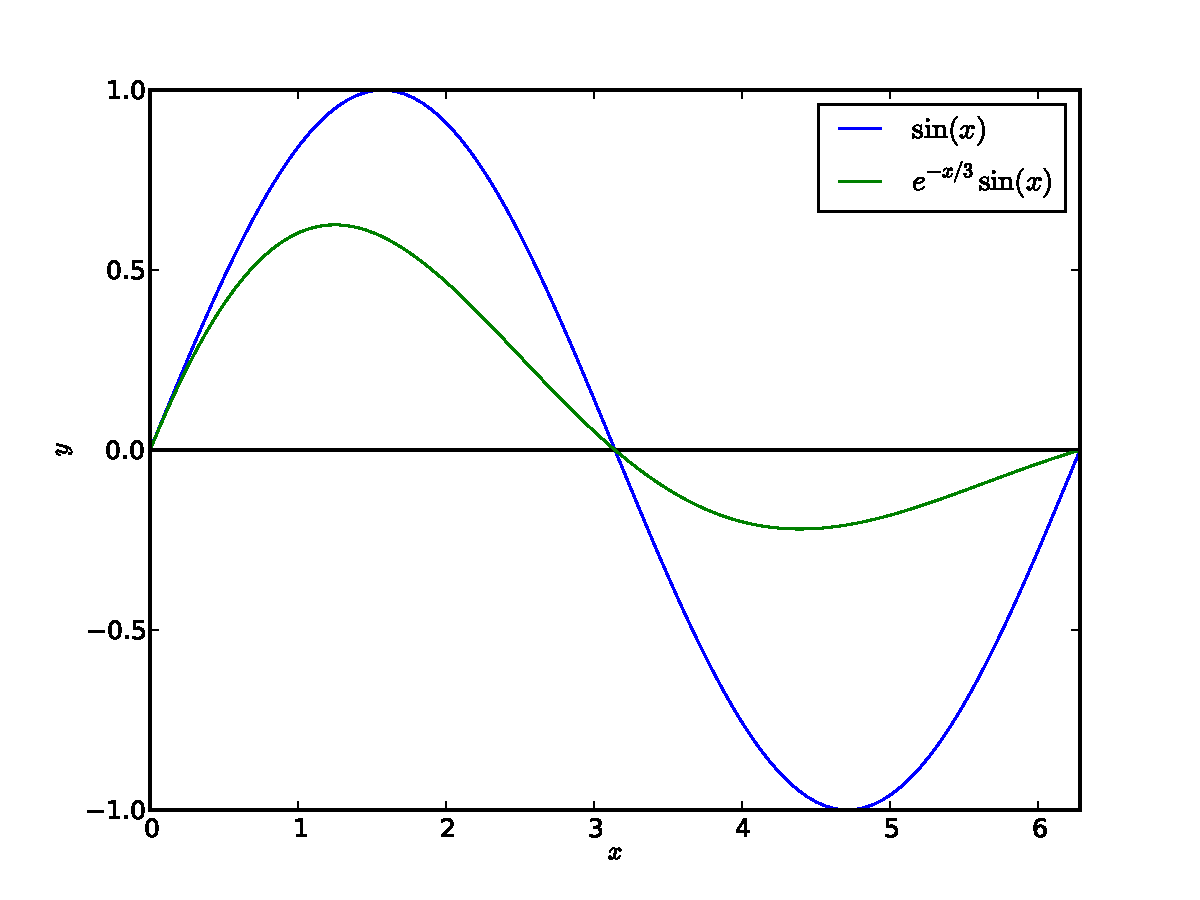
\includegraphics[height=\textwidth]{Chapter-2/figs/sine}
% \caption{This figure has been turned sideways.  With large figures, 
%          the author must ensure that there are at least two double spaces
%          between the caption and the page number.}
% \label{fig:hist}
% \end{figure}
% \end{landscape}
% %\newgeometry{margin=1in,lmargin=1.25in,footskip=\chapterfootskip, includehead, includefoot,landscape=false}
% \restoregeometry
% \pagestyle{fancy}
% \thispagestyle{fancy}
% \newgeometry{margin=1in,lmargin=1.25in,footskip=\chapterfootskip, includehead, includefoot}


% \section{Matrices}
% Let's look at a simple example of a matrix:
% \[ \left( \begin{array}{ccc}
% a & b & c \\
% d & e & f \\
% g & h & i \end{array} \right)\] 
% %
% You may prefer to write it this way:
% \[ \left[\begin{array} {cccccc}
% 1 & 0 & 0 & 0 & 0 & 0 \\
% 0 & 1 & 0 & 0 & 0 & 0 \\
% 0 & 0 & 1 & 0 & 0 & 0 \\
% 0 & 0 & 0 & 1 & 0 & 0 \\
% 0 & 0 & 0 & 0 & 1 & 0 \\
% 0 & 0 & 0 & 0 & 0 & 1 \\
% \end{array} \right] \]
